\chapter{Arrays of Arrays}

The last two chapters of this book will use 2D graphics to illustrate advanced object-oriented concepts.
If you haven't yet read Appendix~\ref{graphics}, please do so now to become familiar with the \java{Canvas}, \java{Color}, and \java{Graphics} classes from the \java{java.awt} package.
We will use these classes to make graphical programs.


\section{Conway's Game of Life}

A mathematician named John Conway invented the ``Game of Life'', which he called a ``zero-player game'' because no players are needed to choose strategies or make decisions.
After you set up the initial conditions, you watch the game play itself.
That turns out to be more interesting than it sounds; you can read about it at \url{http://en.wikipedia.org/wiki/Conways_Game_of_Life}.

\begin{figure}[!ht]
\begin{center}
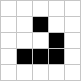
\includegraphics{figs/glider.png}
\caption{A ``Glider'' in the Game of Life.}
\label{fig:glider}
\end{center}
\end{figure}

The game consists of a two-dimensional grid of square cells.
Each cell is either ``alive'' or ``dead''; the color of the call indicates its status.
Figure~\ref{fig:glider} shows an example grid configuration.
The game proceeds in {\bf time steps}, during which every cell interacts with its {\bf neighbors} (adjacent cells).
At each step in time, the following rules are applied:

\begin{enumerate}
\item Any live cell with fewer than two live neighbors dies, as if by underpopulation.
\item Any live cell with more than three live neighbors dies, as if by overpopulation.
\item Any dead cell with exactly three live neighbors becomes a live cell, as if by reproduction.
\end{enumerate}

Notice some consequences of these rules.
If you start with a single live cell, it dies.
If all cells are dead, no cells come to life.
But if you have 4 cells in a square, they keep each other alive; that's a stable configuration.

Most simple starting configurations either die out quickly or reach a stable configuration.
But there are a few starting conditions that display remarkable complexity.
One of those is the R-pentomino: it starts with only five cells, runs for 1103 time steps, and ends in a stable configuration with 116 live cells (see
\url{http://www.conwaylife.com/wiki/R-pentomino}).

In the following sections, we will implement the Game of Life in Java.


\section{The Cell Class}

Using top-down design (see Section~\ref{shuffle}), it's clear we'll need at least three classes: one for the cells, one for the grid, and one for the game itself.
We'll begin by designing the class for cells.

When drawing a cell, we'll need to know its coordinates on the screen.
We could use a \java{Rectangle} object (see Section~\ref{sec:Rectangle}) to store the cell's coordinates.
However, given that the cell is square, we can represent its location with three integers: the \java{x} and \java{y} location of the upper-left corner, and the \java{size} of the square (length of each side).
The cell will also need a \java{Color}.

Here is the beginning of the \java{Cell} class:

\begin{code}
public class Cell {
    private final int x;
    private final int y;
    private final int size;
    private Color color;
}
\end{code}

Notice that \java{x}, \java{y}, and \java{size} are constants.
Once the cell is created, we don't want to move it accidentally.
Its \java{color}, on the other hand, is not a constant and might change frequently.

The next step is to write a constructor.
It's good practice to design classes to be reusable; there are other games that might need to make cells.
We'll make a constructor that takes \java{x}, \java{y}, and \java{size} as parameters.

\begin{code}
public Cell(int x, int y, int size) {
    this.x = x;
    this.y = y;
    this.size = size;
    this.color = Color.WHITE;
}
\end{code}

The following example uses this constructor to create a \java{Cell}.
Its upper-left corner is at (0, 0), and the cell is 10x10 pixels wide.

\begin{code}
Cell cell = new Cell(0, 0, 10);
\end{code}

To draw a cell, we'll receive the graphics context as a parameter (similar to the \java{paint} method in Appendix~\ref{graphics}).
We'll use \java{fillRect} to paint the cell itself and \java{drawRect} to paint a light border around it.

\begin{code}
public void draw(Graphics g) {
    g.setColor(this.color);
    g.fillRect(x + 1, y + 1, size - 1, size - 1);
    g.setColor(Color.LIGHT_GRAY);
    g.drawRect(x, y, size, size);
}
\end{code}

Finally, we will need methods for changing the cell's color.
We could just implement \java{getColor} and \java{setColor}.
But it will be more convenient if we design more specific methods.

For the Game of Life, the cells will either be dead (white) or alive (black).
To make the code reusable, let's refer to these states as ``off'' and ''on''.
We will use class constants to define these colors.

\begin{code}
public static final Color OFF = Color.WHITE;
public static final Color ON = Color.BLACK;

public boolean isOff() {
    return color == OFF;
}

public boolean isOn() {
    return color == ON;
}

public void turnOff() {
    color = OFF;
}

public void turnOn() {
    color = ON;
}
\end{code}


\section{Two-Dimensional Arrays}

